\documentclass{proc-a4}


\begin{document}

\author{A.T. Balkema}

\aff{A.A. Balkema Publishers, Leiden, The Netherlands}

\author{L. Goosen}

\aff{New Institute, Gouda, The Netherlands}

\abstract{Authors of papers to proceedings have to type these in a
form suitable for direct reproduction by the publisher. In order
to ensure uniform style throughout the volume, all the papers have
to be prepared strictly according to the instructions set below.
The enclosed CPI.joboptions should be used to create the final
Camera Ready Copy PDF file. The publisher will reduce the
camera-ready copy to 75\% and print it in black only. For the
convenience of the authors template files for MS Word 6.0 (and
higher) are provided.}

%\keywords{keyword text}

\chapter{Preparing a one column paper with MS-Word for Windows}

\section{GENERAL INSTRUCTIONS}

\subsection{Type area}

The text should fit exactly into the type area (150 � 240 mm). For
A4 size paper the margin settings are: Top: 2.5 cm; Bottom: 3.0
cm; Left: 3.0 cm; Right: 3.0 cm; and all other settings 0.00 cm
(template file: B1ProcA4.dot). For Letter size paper these
settings are: Top: 0.69"; Bottom: 0.79"; Left: 1.29"; Right:
1.29"; and all other settings 0.00" (template file: B1ProcLe.dot).

\subsection{Typefont, typesize and spacing}

Use Times New Roman,  point-size 11 and 12 points line spacing
(Standard;text tag).             Use roman type except for the
headings (Heading tags), parameters in mathematics (not for log,
sin, cos, ln, max., d (in dx), etc), Latin names of species and
genera in botany and zoology and the titles of journals and books
which should all be in italics. Never use bold, except to denote
vectors in mathematics. Never underline any text. Use the small
font (10 points on 11 points) for tables (Table tags), figure
captions (Figure caption tag) and the references (Reference text
tag). Never use letter spacing and never use more than one space
after each other.

\section{GETTING STARTED}

\subsection{The template file}

Copy the template file B1ProcA4.dot (if you print on A4 size
paper) or B1ProcLe.dot (for Letter size paper) to the template
directory. This directory can be found by selecting the Tools
menu,  Options and then by tabbing the File Locations. When the
Word programme has been started open the File menu and choose New.
Now select the template B1ProcA4.dot or B1ProcLe.dot (see above).
Now start by renaming the document by clicking Save As in the menu
Files.


\subsection{Title, author and affiliation frame}

Place the cursor on the T of Title at the top of your newly named
file and type the title of the paper in lower case (no caps except
for proper names). The title should not be longer than 75
characters) . Delete the word Title (do not delete the paragraph
end).

Place the cursor on the A of A.B. Author(s) and type the name of
the first author (first the initials and then the last name). If
any of the co-authors have the same affiliation as the first
author, add his name after an \& (or a comma if more names
follow). Delete the words          A.B. Author etc. and place the
cursor on the A of Affiliation. Type the correct affiliation;
Name of the institute, City, State/Province, Country, do not add
street names, P.O. Box numbers or zip codes to the affiliations.
Now delete the word Affiliation. If there are authors linked to
other institutes, place the cursor at the end of the affiliation
line just typed and give a return. Now type the name(s) of the
author(s) and after a return the affiliation. Repeat this
procedure until all affiliations have been typed.

All the above texts should fit in the frame which should not be
changed (Width: Exactly 15.0 cm or 5,91"; Height: Exactly 7.2 cm
or 2.79"; Lock anchor).

\subsection{Abstract frame}

If there are no further authors place the cursor one space behind
the word ABSTRACT: and type your abstract of not more than 150
words. The first line of the abstract will be 7.2 cm (2.83") from
the top. The complete abstract will fall in the abstract frame,
the settings of which should also not be changed (width: Exactly
15.0 cm or 5.91"; height: Automatic; vertical: 7.2 cm or 2.83"
from margin; Lock anchor).

\subsection{First line of text or heading}

If your text starts with a heading, place the cursor on the I of
INTRODUCTION and type the correct text for the heading. Now delete
the word INTRODUCTION and start with the text    after a return.
This text should have the tag First paragraph.

If your text starts without a heading you should place the cursor
on the I of INTRODUCTION, change the tag to First paragraph and
type your text after deleting the word INTRODUCTION, but not the
return at the end.

\section{LAYOUT OF TEXT}

\subsection{Text and indenting}

All text, figures, tables, etc. should fit exactly in the type
area of 15 � 24 cm (5.91" � 9.52"). All text should be typed in
Times New Roman. All text is 11 pt on 12 pt line spacing except
for the paper title (16 pt on 18 pt), author(s) (12 pt on 13 pt),
affiliation(s) (10 pt on 11 pt) and the small text in tables,
captions and references (10 pt on 11 pt). All line spacing is
exact. Never add a line space between lines or paragraphs.

First lines of paragraphs are indented 4 mm (0.16") except for
paragraphs after a heading or a blank line (First paragraph tag).
Equations are indented 12 mm (0.47") (Formula tag).

\subsection{Headings}

Type primary headings in capital letters roman (Heading 1 tag) and
secondary and tertiary  headings in lower case italics (Headings 2
and 3 tags). Headings are set flush against the left margin. The
tag will give two blank lines (24 pt) above and one (12 pt)
beneath the primary headings, 1� blank lines (18 pt) above and a �
blank line (6 pt) beneath the secondary headings and one blank
line (12 pt) above the tertiary headings. Headings are not
indented and neither are the first lines of text following the
heading indented. If a primary heading is directly followed by a
secondary heading, only a � blank line should be set between the
two headings. In the Word programme this has to be done manually
as follows: Place the cursor on the primary heading, select
Paragraph in the Format menu, and change the setting for spacing
after, from 12 pt to 0 pt. In the same way the setting in the
secondary heading for spacing before should be changed from 18 pt
to 6 pt.

\begin{table}[!h]
\processtable{Margin settings for A4 size paper and letter size
paper.}{
\begin{tabular*}{265pt}{@{\extracolsep\fill}lllll@{}}\toprule
&\multicolumn{2}{c}{A4 size
paper}&\multicolumn{2}{c}{Letter size paper}\\
&\multicolumn{2}{c}{\hrulefill}&\multicolumn{2}{c}{\hrulefill}\\
Setting &cm&inches&cm&inches\\\midrule
Top&2.5&0.98"&1.75&0.69"\\
Bottom&3.0&1.18"&2.01&0.79"\\
Left&3.0&1.18"&3.28&1.29"\\
Right&3.0&1.18"&3.28 &1.29"\\
All other&0.0&0.0"&0.0&0.0"\\\botrule
\end{tabular*}}{}
\end{table}


\subsection{Listing and numbering}

When listing facts use either the style tag List summary signs or
the style tag List number signs.

\subsection{Equations}

Use the equation editor of the selected word processing programme.
Equations are indented 12 mm (0.47") from the left margin (Formula
tag). Number equations consecutively and place the number with the
tab key at the end of the line, between parantheses. Refer to
equations by these numbers. See for example Equation 1 below:

From the above we note that $\sin \theta = (x + y)z$ or:

\begin{equation}
K_t  = \;\left( {1 - \;\frac{{R^2 \tau }}{{c_a  + \nu \;\tan
\;\delta }}} \right)^4 k_1
\end{equation}
where $c_a$ = interface adhesion; $\delta$ = friction angle at
interface; and $k_1$ = shear stiffness number.

\subsection{Tables}

Locate tables close to the first reference to them in the text and
number them consecutively. Avoid abbreviations in column headings.
Indicate units in the line immediately below the heading.
Explanations should be given at the foot of the table, not within
the table itself. Use only horizontal rules: One above and one
below the column headings and one at the foot of the table (Table
rule tag: Use the Shift-minus key to actually type the rule
exactly where you want it). For simple tables use the tab key and
not the table option. Type all text in tables in small type (Table
text tag). Align all headings to the left of their column and
start these headings with an initial capital. Type the caption
above the table to the same width as the table (Table caption
tag). See for example Table 2.

\begin{table}[!h]
\processtable{The number of officially reported plaque cases in
the world.}{
\begin{tabular*}{300pt}{@{\extracolsep\fill}lllllll@{}}\toprule
Region*&1968&1970&1972&1974&1976&1978\\\midrule
Africa&172&27&85&128&183&77\\
America&392&326&301&297&321&142\\
Asia&4395&4111&2312&1408&2230&518\\
Total&4959&4464&2698&1833&2734&737\\\botrule
\end{tabular*}}{*For Europe only one imported case in 1970.}
\end{table}


\subsection{Figure captions}

Always use the Figure caption style tag (10 points size on 11
points line space). Place the      caption underneath the figure
(see Section 5). Type as follows: 'Figure 1. Caption.' Leave about
two lines of space between the figure caption and the text of the
paper.

\begin{figure}
\centering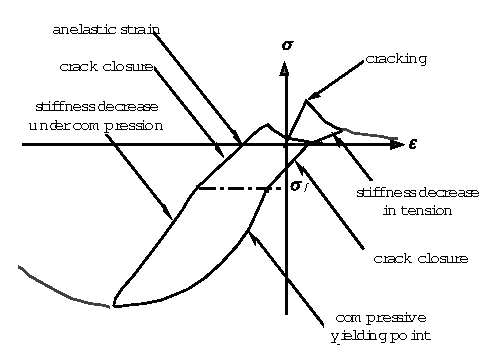
\includegraphics{f1.eps} \caption{Caption of a typical
figure. Photographs will be scanned by the printer. Always supply
original photographs.}
\end{figure}


\subsection{References}

In the text, place the authors' last names (without initials) and
the date of publication in parentheses (see examples in Section
7). At the end of the paper, list all references in alphabetical
order underneath the heading REFERENCES (Heading without number
tag). The references should be typed in small text (10 pt on 11
pt) and second and further lines should be indented 4.0 mm
(Reference text tag). If several works by the same author are
cited, entries should be chronological:

Larch, A.A. 1996a. Development ...

Larch, A.A. 1996b. Facilities ...

Larch, A.A. 1997. Computer ...

Larch, A.A. \& Jensen, M.C. 1996. Effects of ...

Larch, A.A. \& Smith, B.P. 1993. Alpine ...

In bibliographies the order for books and journals are
respectively:

Last name, First name or Initials (ed.) year. {\it Book title}.
City: Publisher.

Last name, First name or Initials year. {\it Title of article}.
Title of Journal (series number if necessary) volume number (issue
number if necessary): page numbers.

Examples:

\begin{thebibliography}{99}

\bibitem{} Grove, A.T. 1980. Geomorphic evolution of the Sahara and the
Nile. In M.A.J. Williams \& H. Faure (eds), {\it The Sahara and
the Nile}: 21-35. Rotterdam: Balkema.

\bibitem{} Jappelli, R. \& Marconi, N. 1997. Recommendations and prejudices
in the realm of foundation engineering in Italy: A historical
review. In Carlo Viggiani (ed.), {\it Geotechnical engineering for
the preservation of monuments and historical sites; Proc. intern.
symp., Napoli, 3-4 October 1996}. Rotterdam: Balkema.

\bibitem{} Johnson, H.L. 1965. Artistic development in autistic children.
{\it Child Development} 65(1): 13-16. Polhill, R.M. 1982. {\it
Crotalaria in Africa and Madagascar}. Rotterdam: Balkema.
\end{thebibliography}

\subsection{Notes}

These should be avoided. Insert the information in the text. In
tables the following reference marks should be used: *, **, etc.
and the actual footnotes are set directly underneath the table.

\subsection{Conclusions}

Conclusions should state concisely the most important propositions
of the paper as well as the author's views of the practical
implications of the results.

\section{PHOTOGRAPHS AND FIGURES}

Number figures consecutively in the order in which reference is
made to them in the text, making no distinction between diagrams
and photographs. Figures should fit within the column width of 90
mm (3.54") or within the type area width of 187 mm (7.36").

Figures, photographs, etc. should be in black only. Paste copies
of the same size onto the typescript where you want them to appear
in the text. Do not place them sideways on a page. Figures, etc.
should not be centered, but placed against the left margin. Leave
about two lines of space between the actual text and figure
(including caption). Never place any text next to a figure. Leave
this space blank. The most convenient place for placing figures is
at the top or bottom of the page. Avoid placing text between
figures as readers might not notice the text. Line drawings (as
well as photographic reproductions of these) should be in black
(not grey) on white. Keep in mind that everything will be reduced
to 75\%. Therefore, 9 point should be the minimum size of the
lettering. Lines should preferably be 0.2 mm (0.1") thick. Keep
figures as simple as possible. Avoid excessive notes and
designations.

\section{PREFERENCES, SYMBOLS AND UNITS}

Consistency of style is very important. Note the spacing,
punctuation and caps in all the examples below.

\begin{itemize}
\item[--]   References in the text: Figure 1, Figures 2-4, 6, 8a, b
(not abbreviated)
\item[--] References between parentheses: (Fig. 1),
(Figs 2-4, 6, 8a, b) (abbreviated)
\item[--] USA / UK / The Netherlands
instead of U.S.A. / U.K. / Netherlands / the Netherlands
\item[--] Author
\& Author (1989) instead of Author and Author (1989)
\item[--] (Author
1989a, b, Author \& Author 1987) instead of (Author, 1989a,b;
Author and Author, 1987)
\item[--] (Author et al. 1989) instead of
(Author, Author \& Author 1989)
\item[--]Use the following style:
(Author, in press); (Author, in prep.); (Author, unpubl.);
(Author, pers. comm.)
\end{itemize}

Always use the official SI notations:

\begin{itemize}
\item[--] kg / m / kJ / cm {\it instead of} kg. (Kg) / m. / kJ. (KJ) / cm.;
\item[--] 20$^\circ$16$^\prime$32$^\prime$$^\prime$SW {\it instead of} 20$^\circ$ 16$^\prime$
32$^{\prime\prime}$ SW
\item[--]   0.50 {\it instead of} 0,50 ({\it used in French text}); 9000 {\it instead
of} 9,000 {\it but if more than} 10,000: 10,000 {\it instead of}
10000
\item[--]   ${}^{14}C$ {\it instead of} $C^{14}$ / C-14 {\it and} BP / BC / AD {\it instead of} B.P. /
B.C. / A.D.
\item[--]   20 {\it instead of} $\times$20 / X20 / x 20; 4 + 5 > 7 {\it instead of} 4+5>7 {\it
but} -8 / +8 {\it instead of} - 8 / + 8
\item[--] e.g. / i.e. {\it instead of} e.g., / i.e.,
\end{itemize}

\section{SUBMISSION OF MATERIAL TO THE EDITOR}

The camera-ready copy PDF file of the complete paper should be
created with the enclosed CPI.joboptions file and sent to the
editor. All figures should be included as high resolution file in
the PDF file (see artwork document). Check whether the paper looks
the same as this sample: Title at top of first page in 18 points,
authors in 14 points and all other text in 12 points on 13 points
line space, except for the small text (10 point on 11 point line
space) used in tables, captions and references. Also check if the
type width is 187 mm (7.36"), the column width 90 mm (3.54"), the
page length is 272 mm (10.71") and that the space above the
Abstact is exactly as in the sample.

\end{document}
